\documentclass{standalone}
\usepackage{tikz}
\usepackage{verbatim}
\begin{document}
\pagestyle{empty}
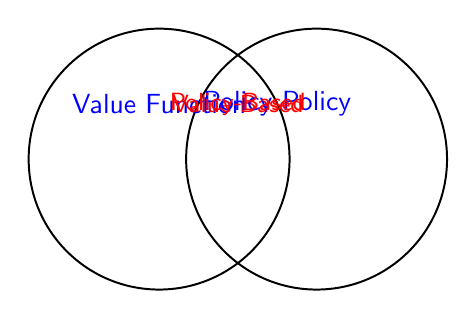
\begin{tikzpicture}
\node[draw,circle,scale=10., fill=none, line width=0.25mm] at (-1.,0) {};
\node[draw,circle,scale=10., fill=none, line width=0.25mm] at (1.,0) {};
\node[font=\sffamily] at (-1.,0.7) {\color{blue}Value Function};
\node[font=\sffamily] at (1.,0.7) {\color{blue}Policy};

\node[font=\sffamily] at (0.,0.7) {\small\color{red}Value Based};
\node[font=\sffamily] at (0.,0.7) {\color{blue}Policy};
\node[font=\sffamily] at (0.,0.7) {\small\color{red}Policy-Based};
\end{tikzpicture}
\end{document}